\documentclass[a4paper,12pt]{article}
\pdfoutput=1
\usepackage{epsfig}
\usepackage{amssymb}
\usepackage{amsfonts}
\usepackage{mathtools, physics}
\usepackage{euscript}
\usepackage{verbatim}
\usepackage{latexsym}
\usepackage{graphicx}
\usepackage{caption}
\usepackage{float}
%\usepackage{svg}
\usepackage{subcaption}
\usepackage[hidelinks]{hyperref}
\usepackage{multicol}
\usepackage{listings}
\usepackage{tabularx, adjustbox, diagbox, booktabs, makecell, array, multirow}
\usepackage{siunitx}
\usepackage[none]{hyphenat}

\graphicspath{ {./figures/} }

\usepackage{import}
\usepackage{xifthen}
\usepackage{pdfpages}
\usepackage{transparent}
\newcommand{\incfig}[1]{%
    \def\svgwidth{\columnwidth}
    \import{./figures/}{#1.pdf_tex}
}

%\usepackage{mathabx}
%\usepackage{wrapfig}
%	\usepackage[T1]{fontenc}
%	\usepackage{tikz}
%	\usetikzlibrary{decorations.pathmorphing}
%\usepackage{tikz}
%\usetikzlibrary{shapes.geometric, arrows,patterns,snakes}
%\tikzstyle{ellip} = [ellipse, minimum width=3cm, minimum height=1cm,text centered, draw=black]

%\newskip\humongous \humongous=0pt plus 1000pt minus 1000pt
\def\caja{\mathsurround=0pt}
\def\eqalign#1{\,\vcenter{\openup1\jot \caja
 \ialign{\strut \hfil$\displaystyle{##}$&$
 \displaystyle{{}##}$\hfil\crcr#1\crcr}}\,}
\newif\ifdtup
\def\panorama{\global\dtuptrue \openup1\jot \caja
 \everycr{\noalign{\ifdtup \global\dtupfalse
 \vskip-\lineskiplimit \vskip\normallineskiplimit
 \else \penalty\interdisplaylinepenalty \fi}}}
\def\eqalignno#1{\panorama \tabskip=\humongous
 \halign to\displaywidth{\hfil$\displaystyle{##}$
 \tabskip=0pt&$\displaystyle{{}##}$\hfil
 \tabskip=\humongous&\llap{$##$}\tabskip=0pt
 \crcr#1\crcr}}


%%%%%%%%%%%%%%%%%%%%%%%%%%%%%%%%%%%%%%%%%%%%%%%
\jot = 1.5ex
\def\baselinestretch{1.2}
\parskip 3pt plus 1pt

\catcode`\@=11

\@addtoreset{equation}{section}
\def\theequation{\thesection.\arabic{equation}}

\def\@normalsize{\@setsize\normalsize{15pt}\xiipt\@xiipt
\abovedisplayskip 14pt plus3pt minus3pt%
\belowdisplayskip \abovedisplayskip
\abovedisplayshortskip \z@ plus3pt%
\belowdisplayshortskip 7pt plus3.5pt minus0pt}

\def\small{\@setsize\small{13.6pt}\xipt\@xipt
\abovedisplayskip 13pt plus3pt minus3pt%
\belowdisplayskip \abovedisplayskip
\abovedisplayshortskip \z@ plus3pt%
\belowdisplayshortskip 7pt plus3.5pt minus0pt
\def\@listi{\parsep 4.5pt plus 2pt minus 1pt
     \itemsep \parsep
     \topsep 9pt plus 3pt minus 3pt}}

\relax


\catcode`@=12


\topmargin -.5cm
\textheight 23cm
\hoffset-1cm
\textwidth 16.5cm


\catcode`\@=11

\def\section{\@startsection{section}{1}{\z@}{3.5ex plus 1ex minus
   .2ex}{2.3ex plus .2ex}{\large\bf}}


\def\YGrule{0.4}   
\def\YGbox{6.5}    
\def\SymBoxes#1#2#3#4{\newdimen\un@t \un@t#3%
\raisebox{#1}{\rule{#2\un@t}{#4}\hskip-#2\un@t% lower horizontal
\@tempdimb\un@t \advance\@tempdimb by-#4\@tempcntb#2\relax%
\@whilenum{\@tempcntb>0}\do{%                         % #2 vertical lines
\rule{#4}{\un@t}\hskip\@tempdimb \advance\@tempcntb by\m@ne}%
\hskip-#2\un@t \rule[\un@t]{#2\un@t}{#4}%
\rule[\un@t]{#4}{#4}\hskip-#4%             % upper horizontal line
\rule{#4}{\un@t}}\hskip-#4}                % rightest vertical line
%                                         %(over)draw symmetric boxes next
%%%%%%%%%




\begin{document}
%\begin{letter}{~}
\sloppy

%%%%%%Define some new commands and  macros
\newcommand{\beq}{\begin{equation}}
\newcommand{\eeq}{\end{equation}}
\newcommand{\bea}{\begin{eqnarray}}
\newcommand{\eea}{\end{eqnarray}}
\newcommand{\beas}{\begin{eqnarray*}}
\newcommand{\eeas}{\end{eqnarray*}}
\newcommand{\defi}{\stackrel{\rm def}{=}}
\newcommand{\non}{\nonumber}
\newcommand{\bquo}{\begin{quote}}
\newcommand{\enqu}{\end{quote}}
%%%%%%%%%%%%%%%%
\renewcommand{\(}{\begin{equation}}
\renewcommand{\)}{\end{equation}}
%%%%%%%%%%%%%%%%%%%%%%%%%%%%%%%%%% definitions
\def \eqn#1#2{\begin{equation}#2\label{#1}\end{equation}}

\def\e{\epsilon}
\def\IZ{{\mathbb Z}}
\def\IR{{\mathbb R}}
\def\IC{{\mathbb C}}
\def\IQ{{\mathbb Q}}
\def\IH{{\mathbb H}}
\def\de{\partial}
\def\Tr{ \hbox{\rm Tr}}
\def\H{ \hbox{\rm H}}
\def\HE{ \hbox{$\rm H^{even}$}}
\def\HO{ \hbox{$\rm H^{odd}$}}
\def\K{ \hbox{\rm K}}
\def\Im{ \hbox{\rm Im}}
\def\Ker{ \hbox{\rm Ker}}
\def\const{\hbox {\rm const.}}
\def\o{\over}
\def\im{\hbox{\rm Im}}
\def\re{\hbox{\rm Re}}
\def\bra{\langle}\def\ket{\rangle}
\def\Arg{\hbox {\rm Arg}}
\def\Re{\hbox {\rm Re}}
\def\Im{\hbox {\rm Im}}
\def\exo{\hbox {\rm exp}}
\def\diag{\hbox{\rm diag}}
\def\longvert{{\rule[-2mm]{0.1mm}{7mm}}\,}
\def\a{\alpha}
\def\dag{{}^{\dagger}}
\def\tq{{\widetilde q}}
\def\p{{}^{\prime}}
\def\W{W}
\def\N{{\cal N}}
\def\hsp{,\hspace{.7cm}}

\def\br{\nonumber}
\def\IZ{{\mathbb Z}}
\def\IR{{\mathbb R}}
\def\IC{{\mathbb C}}
\def\IQ{{\mathbb Q}}
\def\IP{{\mathbb P}}
\def \eqn#1#2{\begin{equation}#2\label{#1}\end{equation}}


\newcommand{\C}{\ensuremath{\mathbb C}}
\newcommand{\Z}{\ensuremath{\mathbb Z}}
\newcommand{\R}{\ensuremath{\mathbb R}}
\newcommand{\rp}{\ensuremath{\mathbb {RP}}}
\renewcommand{\cp}{\ensuremath{\mathbb {CP}}}
\newcommand{\vac}{\ensuremath{|0\rangle}}
\newcommand{\vact}{\ensuremath{|00\rangle}                    }
\newcommand{\oc}{\ensuremath{\overline{c}}}
\newcommand{\psizero}{\psi_{0}}
\newcommand{\phizero}{\phi_{0}}
\newcommand{\hzero}{h_{0}}
\newcommand{\psiin}{\psi_{\rh}}
\newcommand{\phiin}{\phi_{\rh}}
\newcommand{\hin}{h_{\rh}}
\newcommand{\rh}{r_{h}}
\newcommand{\rb}{r_{b}}
\newcommand{\psibnd}{\psi_{0}^{b}}
\newcommand{\psibndp}{\psi_{1}^{b}}
\newcommand{\phibnd}{\phi_{0}^{b}}
\newcommand{\phibndp}{\phi_{1}^{b}}
\newcommand{\gbnd}{g_{0}^{b}}
\newcommand{\hbnd}{h_{0}^{b}}
\newcommand{\zh}{z_{h}}
\newcommand{\zb}{z_{b}}
\newcommand{\man}{\mathcal{M}}
\newcommand{\hbr}{\bar{h}}
\newcommand{\tbr}{\bar{t}}

\renewcommand{\d}[1]{\text{d} #1}
\newcommand{\B}[1]{\boldsymbol{#1}}
\newcommand{\vv}{\\[0.1ex] &\hspace{0.5cm}}


\begin{titlepage}
\begin{flushright}
CHEP XXXXX
%ULB-TH/09-10\\
%hep-th/yymmnnn\\
\end{flushright}
\bigskip
\def\thefootnote{\fnsymbol{footnote}}

\begin{center}
{\Large
{\bf Field theories on the boundary of Minkowski space
%\vspace{0.15in}
%Geometrizing the Flat Space Information Paradox
}
}
\end{center}
\begin{center}
% {\small Essay written for the Gravity Research Foundation 2021 Awards for Essays on Gravitation\\ Submission Date: March 31st, 2021 \\ }

\bigskip

Chethan KRISHNAN$^a$\footnote{\texttt{chethan.krishnan@gmail.com}}
Rishi Raj$^b$\footnote{\texttt{rishiraj.1012exp@gmail.com}}
\vspace{0.1in}

\end{center}

\renewcommand{\thefootnote}{\arabic{footnote}}


\begin{center}


$^a$ {Center for High Energy Physics,\\
Indian Institute of Science, Bangalore 560012, India}\\

$^b$ {Department of Physics, \\
Indian Institute of Technology Madras, Chennai 600036, India}\\

\end{center}

\noindent
\begin{center} {\bf Abstract} \end{center} 

Stuff goes here...


\vspace{1.6 cm}
\vfill

\end{titlepage}

\setcounter{footnote}{0}

%%%%%%%%%%%%%%%%%%%%%%%%%%%%%%%%%%%%%%%%%%%%%%%%%%%%%%%%%%%%%%%%%%%%%%%%%%%%%%%%%%%%%%%%%%%%%%
%%%%%%%%%%%%%%%%%%%%%%%%%%%%%%%%%%%%%%%%%%%%%%%%%%%%%%%%%%%%%%%%%%%%%%%%%%%%%%%%%%%%%%%%%%%%%%
\section{Introduction}

XXXXXeevefnnlel


\section{Allowed Fine-Tunings?}



Even though 

Our observations  

\section{Acknowledgments}

We thank ...

\appendix

\section{AdS and Minkowski space}

   One way to define the various AdS spaces is through an embedding in a higher dimensional flat space (Lorenzian AdS in a flat space with two time directions and Euclidean AdS on Minkowski space). Specifically, one defines (Lorenzian) $\text{AdS}_{d+1}$ as the following algebraic set
   \begin{equation}\label{eqn:ads-definition}
      \text{AdS}_{d+1} \coloneqq \{ (X^{-1}, X^{0}, \ldots X^{d}) \in \mathbb{R}^{d, 2} \mid \eta_{A B} X^A X^B = -L^2 \}
   \end{equation}
   where $\eta = \diag (-1, -1, 1, \ldots 1)$ is the canonical metric on $\mathbb{R}^{d, 2}$ and $L$ is a positive real number which sets a length scale on this space (called the AdS length scale). The set above derives its topology, smooth structure and pseudo-Riemmanian structure from that of its ambient space. 
   
   Another interesting property of this space is that it's (conformal) boundary (note that the space above is not a manifold with boundary, we speak of its conformal boundary) is a flat Minkowski space of one lower dimension. To see this, set $X^A = s \, x^A$ and take the limit $s \to \infty$. The set $\partial (\text{AdS}_{d+1})$ obtained this way is
   \begin{equation}\label{eqn:ads-boundary}
      \partial (\text{AdS}_{d+1}) =\{ [x^{-1}, x^{0}, \ldots x^{d}] \in \mathbb{RP}^{d+1} \mid \eta_{A B} x^A x^B = -\frac{L^2}{s^2} \to 0 \}
   \end{equation}
   In other words, the set of points with $(x^{-1})^2 + (x^{0})^2 = (x^1)^2 + \ldots + (x^d)^2$. In addition, there is an overall scale equivalence ($x^A \sim c \, x^A$, where, importantly, $c$ can be negative) because of the above construction (hence $\mathbb{RP}^{d+1}$ and not $\mathbb{R}^{d, 2}$). Thus, to fix this ambiguity, one can always take $(x^{-1})^2 + (x^{0})^2 = (x^1)^2 + \ldots + (x^d)^2 = 1$ (with the remaining identification of $x^A$ and $-x^A$). This space is topologically $\boldsymbol{S}^1 \times \boldsymbol{S}^{d-1} / \mathbb{Z}_2$ and has closed timelike curves. It is, in fact, a compactification of Minkowski space $\mathbb{R}^{d-1,1}$. One "unfolds" the time circle to get the universal cover $\mathbb{R} \times \boldsymbol{S}^{d-1}$. 
   
   To see how \ref{eqn:ads-boundary} is $\mathbb{R}^{d-1,1}$, write $u = X^{-1} - X^d$ and $v = X^{-1} + X^d$. The set in \ref{eqn:ads-boundary} then is the locus $-uv + \sum_{i j} \eta_{i j} x^i x^j = 0$. Here $\eta_{i j}$ is the metric on $\mathbb{R}^{d-1,1}$ with coordinates $(x^0, \ldots x^{d-1})$. If we ignore the measure zero set $v=0$, one can set it equal to one by scale equivalence and get $u$ as a function of of the $x^i$ which is just Minkowski space.
   
   Another important property of the two sets defined above is that they have a natural action of $\mathit{SO}(d, 2)$ from the ambient space. Indeed, it is not hard to see that this is the full isometry group of $\text{AdS}_{d + 1}$ (since the other isometries of $\mathbb{R}^{d, 2}$, translations, don't leave this set invariant). For the compactified Minkowski space \ref{eqn:ads-boundary}, this is the group of comformal isometries. This makes immediate sense since the boundary is a conformally defined strucure.

   \subsection{Coordinates on AdS}
      An obvious way to construct a coordinate chart for the set \ref{eqn:ads-definition} is
      \begin{align}
         X^{-1} &= L \, \cosh \rho \, \cos \tau \cr
         X^{0} &= L \, \cosh \rho \, \sin \tau \cr
         X^{a} &= L \, \sinh \rho \, y^{a} \hspace{0.05\linewidth} a = 1, \ldots, d
      \end{align}
      where $y^a$ are coordinates on the sphere $\boldsymbol{S}^{d-1}$ (e.g. ultraspherical coordinates). These are called \textbf{global} coordinates because the global (topological) structure of $\text{AdS}_{d+1}$ is manifest in them. Note that the ``time'' coordiate $\tau$ is ``unfolded'' (takes values in all of $\mathbb{R}$). The induced metric on this space can now be easily written.
      \begin{equation}
         \d{s}^2 = \eta_{A B} \pdv{X^A}{u^a} \pdv{X^B}{u^b} \d{u}^a \d{u}^b = L^2 (-\cosh^2\rho \, \d{\tau}^2 + \d{\rho}^2 + \sinh^2\rho \, \d{\Omega}_{d-1}^2)
      \end{equation}

      The boundary in these coordinates corresponds to $\rho \to \infty$. One can ``bring'' the boundary (not at a closer distance but at finite values of the coordinates) by changing to a \textbf{trigonometric version} of global coordinates defined by $\sinh \rho = \tan \eta$. (The intuition here is simple, $\cosh^2\rho - \sinh^2\rho = 1$ but also $\sec^2\eta - \tan^2\eta = 1$). The metric in these coordinates is
      \begin{equation}
         \d{s}^2 = \frac{L^2}{\cos^2\eta} (-\d{\tau}^2 + \d{\eta}^2 + \sin^2\eta \, \d{\Omega}_{d-1}^2)
      \end{equation}
      And indeed, the boundary is now at $\eta \to \frac{\pi}{2}$. In fact, these coordinates give AdS it's usual picture as a cylinder (for $\text{AdS}_3$, see \autoref{fig:ads3})
      \begin{figure}[H]
         \centering
         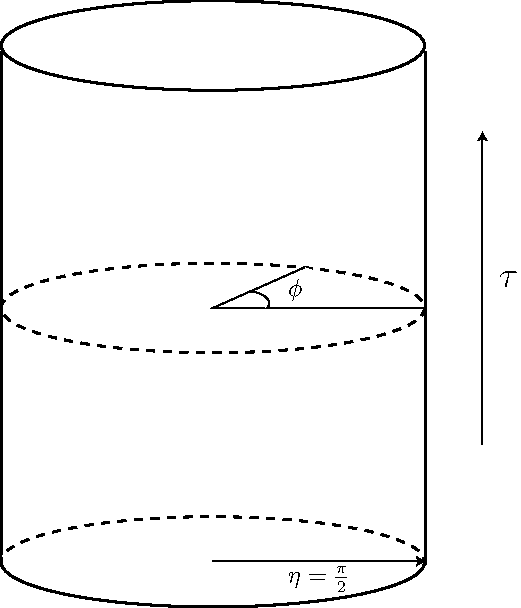
\includegraphics[width=0.5\linewidth]{cylinder.pdf}
         \caption{$\text{AdS}_3$ in trigonometric global coordinates}
         \label{fig:ads3}
      \end{figure}

      Another convenient set of coordinates is the \textbf{area gauge}. The idea is to make the volume of the $(d-1)$-sphere equal to it's usual volume. It's easy to see that $r = L \sinh \rho$ does the job. The metric in these coordinates read (with another tiny change $t = L \, \tau$)
      \begin{equation}
         \d{s}^2 = - (1 + \frac{r^2}{L^2}) \, \d{t}^2 + \frac{\d{r}^2}{(1 + \frac{r^2}{L^2})} + r^2 \, \d{\Omega}_{d-1}^2
      \end{equation}

      One can further define a \textbf{tortoise coordinate} $r^*$ to simplify the radial null directions
      \begin{equation}
         r^* = \int \frac{\d{r}}{(1 + \frac{r^2}{L^2})} = L \tan^{-1}\frac{r}{L} \hspace{0.05\linewidth} \d{s}^2 = \sec^2 \frac{r^*}{L} \, ( -\d{t}^2 +  \d{r^{\ast 2}} ) + L^2 \tan^2 \frac{r^{\ast}}{L} \, \d{\Omega}_{d-1}^2
      \end{equation}
      which is exactly the same as the trigonometric global coordinates above (with $\eta = \frac{r^*}{L}$).

      To further simplify the null directions we can also go to forward or backwards Eddington-Finklestein coordinates or directly jump to the \textbf{Bondi} or \textbf{double-null} gauge ($u$, $v$, $y^a$)
      \begin{align}
         u &= t - r^* \cr
         v &= t + r^* \cr
         \d{s}^2 &= - \sec^2 \frac{v-u}{2 L} \, \d{u} \, \d{v} + L^2 \tan^2 \frac{v-u}{2 L} \, \d{\Omega}_{d-1}^2
      \end{align}

      Another extremely useful gauge is the \textbf{Poincare patch}. Most formulations of AdS/CFT correspondence use this gauge since the Minkowski structure of the boundary is manifest in them. To derive them, one works in ``light-cone'' coordinates on the ambient space.
      \begin{align}
         X^+ &= X^{-1} + X^d \cr
         X^- &= X^{-1} - X^d \cr
         X^\mu &\hspace{0.05\linewidth} \mu = 0, 1, \ldots d-1
      \end{align}
      $\text{AdS}_{d+1}$ is now (the locus of) $-X^{+}X^{-} + \eta_{\mu \nu} X^\mu X^\nu = -L^2$. Where $(\eta_{\mu \nu}) = \diag (-1, 1, \ldots, 1)$.
      After a bit of thought, one can arrive at the following parametrization
      \begin{align}
         X^{+} &= z + \frac{x^\mu x_\mu}{z} \cr
         X^{-} &= \frac{L^2}{z} \cr
         X^{\mu} &= \frac{L}{z} x^\mu
      \end{align}
      The metric in these coordinates takes the simple form
      \begin{equation}
         \d{s}^2 = \frac{L^2}{z^2} \, (\d{z}^2 + \d{x}^\mu \d{x}_\mu)
      \end{equation}
      Note that the conformal boundary is now at $z \to 0$ which is not part of the manifold. But this forces us to choose either $z > 0$ or $z < 0$. Therefore, these coordinates divide the space into two ``patches'' (hence the name) joined in between by the boundary.
      Note how it is clearly evident that the boundary is Minkowski space with global inertial coordinates $x^\mu$.

   \subsection{AdS Isometries and Killing vectors}
      From the argument about isometries earlier, it is clear that the Killing vectors of $\text{AdS}_{d+1}$ are the Lorentz generators $\B{J}_{A B} \in \text{T}_{p} \mathbb{R}^{d, 2}$ of the ambient space projected down to \ref{eqn:ads-definition}. (I write tangent vector fields in bold)
      \begin{equation}
         \B{J}_{A B} = X_A \B{\partial}_B - X_B \B{\partial}_A
      \end{equation}
      The projection is a simple pullback
      \begin{equation}
         \B{j}_{A B} = (\iota_* \, \B{J}_{A B}^{\flat})^{\sharp} = g^{-1}( \iota_* \, \eta(\B{J}_{A B}, -), -)
      \end{equation}
      of the embedding/inclusion map $\iota \colon \text{AdS}_{d+1} \to \mathbb{R}^{d, 2}$. In coordinates, this is (assuming $u^i$ are coordinates on AdS, like one of the above)
      \begin{align}
         \B{j}_{A B}^{k} &= g^{k i} \pdv{X^C}{u^i} \eta_{C D} \B{J}_{A B}^{D} \B{}
      \end{align}
      It is straightforward to calculate this for the various coordinate systems described above.
      Below, I do this for $\text{AdS}_3$ for simplicity.

      \subsubsection{Global coordinates \texorpdfstring{$(\rho, \tau, \phi)$}{}}
         % \begin{align*}
         %    \text{Metric} \hspace{0.05\linewidth}& \d{s}^2 = L^2 (-\cosh^2\rho \, \d{\tau}^2 + \d{\rho}^2 + \sinh^2\rho \, \d{\Omega}_{d-1}^2) \\
         %    \text{Boundary} \hspace{0.05\linewidth}& \rho \to \infty
         % \end{align*}
         % \newcolumntype{A}{ >{$} r <{$} }
         % \begin{table}[H]
         %    \centering
         %    \begin{tabular}{\textwidth}{lAA}
         %       \toprule
         %       Killing vector & \text{On bulk} & \text{On boundary} \\
         %       \midrule
         %       $\B{j}_{-1 0}$ & -\cos (\tau ) \cos (\phi) + \tanh (\rho ) \sin (\tau ) \cos (\phi ) + \coth (\rho ) \cos (\tau ) \sin (\phi ) & -\cos (\tau ) \cos (\phi) + \tanh (\rho ) \sin (\tau ) \cos (\phi ) + \coth (\rho ) \cos (\tau ) \sin (\phi) \\
         %       \bottomrule
         %    \end{tabular}
         %    \label{tab:global-killing}
         % \end{table}
         \begin{align}
            \text{\textbf{Metric}} &\quad \d{s}^2 = L^2 (-\cosh^2\rho \, \d{\tau}^2 + \d{\rho}^2 + \sinh^2\rho \, \d{\phi}^2) \\
            \text{\textbf{Boundary}} &\quad \rho \to \infty
         \end{align}
         \begin{table}[H]
            \centering
            \begin{adjustbox}{width=0.80\textwidth}
               \small
               \begin{tabular}{ccc}
                  \toprule
                     Killing vector & On Bulk & On Boundary \\
                  \midrule
                     $\B{j}_{-1 0}$ & $-\B{\partial}_\tau$ & $-\B{\partial}_\tau$ \\
                     $\B{j}_{-1 1}$ & \parbox{0.3\textwidth}{\begin{equation*}
                        \begin{split}
                           -\cos\tau \cos\phi \, \B{\partial}_\rho \\ + \tanh\rho \sin\tau \cos\phi \, \B{\partial}_\tau \\ + \coth\rho \cos\tau \sin\phi \, \B{\partial}_\phi 
                        \end{split}
                     \end{equation*}} & \parbox{0.3\textwidth}{\begin{equation*}
                        \begin{split}
                           \sin\tau \cos\phi \, \B{\partial}_\tau \\ + \cos\tau \sin\phi \, \B{\partial}_\phi 
                        \end{split}
                     \end{equation*}} \\
                     $\B{j}_{-1 2}$ & \parbox{0.3\textwidth}{\begin{equation*}
                        \begin{split}
                           -\cos\tau \sin\phi \, \B{\partial}_\rho \\ + \tanh\rho \sin\tau \sin\phi \, \B{\partial}_\tau \\ - \coth\rho \cos\tau \cos\phi \, \B{\partial}_\phi 
                        \end{split}
                     \end{equation*}} & \parbox{0.3\textwidth}{\begin{equation*}
                        \begin{split}
                           \sin\tau \sin\phi \, \B{\partial}_\tau \\ - \cos\tau \cos\phi \, \B{\partial}_\phi 
                        \end{split}
                     \end{equation*}} \\
                     $\B{j}_{0 1}$ & \parbox{0.3\textwidth}{\begin{equation*}
                        \begin{split}
                           -\sin\tau \cos\phi \, \B{\partial}_\rho \\ - \tanh\rho \cos\tau \cos\phi \, \B{\partial}_\tau \\ + \coth\rho \sin\tau \sin\phi \, \B{\partial}_\phi 
                        \end{split}
                     \end{equation*}} & \parbox{0.3\textwidth}{\begin{equation*}
                        \begin{split}
                           -\cos\tau \cos\phi \, \B{\partial}_\tau \\ + \sin\tau \sin\phi \, \B{\partial}_\phi 
                        \end{split}
                     \end{equation*}} \\
                     $\B{j}_{0 2}$ & \parbox{0.3\textwidth}{\begin{equation*}
                        \begin{split}
                           -\sin\tau \sin\phi \, \B{\partial}_\rho \\ - \tanh\rho \cos\tau \sin\phi \, \B{\partial}_\tau \\ - \coth\rho \sin\tau \cos\phi \, \B{\partial}_\phi 
                        \end{split}
                     \end{equation*}} & \parbox{0.3\textwidth}{\begin{equation*}
                        \begin{split}
                           -\cos\tau \sin\phi \, \B{\partial}_\tau \\ - \sin\tau \cos\phi \, \B{\partial}_\phi 
                        \end{split}
                     \end{equation*}} \\
                     $\B{j}_{1 2}$ & $\B{\partial}_\phi$ & $\B{\partial}_\phi$ \\
                  \bottomrule
               \end{tabular}
            \end{adjustbox}
         \end{table}


         \subsubsection{Trigonometric global coordinates (also in tortoise coordinates) \texorpdfstring{$(\eta, \tau, \phi)$}{}}
         \begin{align}
            \text{\textbf{Metric}} &\quad \d{s}^2 = \frac{L^2}{\cos^2\eta} (-\d{\tau}^2 + \d{\eta}^2 + \sin^2\eta \, \d{\phi}^2) \\
            \text{\textbf{Boundary}} &\quad \eta \to \frac{\pi}{2}
         \end{align}
         \begin{table}[H]
            \centering
            \begin{adjustbox}{width=0.80\textwidth}
               \small
               \begin{tabular}{ccc}
                  \toprule
                     Killing vector & On Bulk & On Boundary \\
                  \midrule
                     $\B{j}_{-1 0}$ & $-\B{\partial}_\tau$ & $-\B{\partial}_\tau$ \\
                     $\B{j}_{-1 1}$ & \parbox{0.3\textwidth}{\begin{equation*}
                        \begin{split}
                           -\cos\eta \cos\tau \cos\phi \, \B{\partial}_\rho \\ + \sin\eta \sin\tau \cos\phi \, \B{\partial}_\tau \\ + \csc\eta \cos\tau \sin\phi \, \B{\partial}_\phi 
                        \end{split}
                     \end{equation*}} & \parbox{0.3\textwidth}{\begin{equation*}
                        \begin{split}
                           \sin\tau \cos\phi \, \B{\partial}_\tau \\ + \cos\tau \sin\phi \, \B{\partial}_\phi 
                        \end{split}
                     \end{equation*}} \\
                     $\B{j}_{-1 2}$ & \parbox{0.3\textwidth}{\begin{equation*}
                        \begin{split}
                           -\cos\eta \cos\tau \sin\phi \, \B{\partial}_\rho \\ + \sin\eta \sin\tau \sin\phi \, \B{\partial}_\tau \\ - \csc\eta \cos\tau \cos\phi \, \B{\partial}_\phi 
                        \end{split}
                     \end{equation*}} & \parbox{0.3\textwidth}{\begin{equation*}
                        \begin{split}
                           \sin\tau \sin\phi \, \B{\partial}_\tau \\ - \cos\tau \cos\phi \, \B{\partial}_\phi 
                        \end{split}
                     \end{equation*}} \\
                     $\B{j}_{0 1}$ & \parbox{0.3\textwidth}{\begin{equation*}
                        \begin{split}
                           -\cos\eta \sin\tau \cos\phi \, \B{\partial}_\rho \\ - \sin\eta \cos\tau \cos\phi \, \B{\partial}_\tau \\ + \csc\eta \sin\tau \sin\phi \, \B{\partial}_\phi 
                        \end{split}
                     \end{equation*}} & \parbox{0.3\textwidth}{\begin{equation*}
                        \begin{split}
                           -\cos\tau \cos\phi \, \B{\partial}_\tau \\ + \sin\tau \sin\phi \, \B{\partial}_\phi 
                        \end{split}
                     \end{equation*}} \\
                     $\B{j}_{0 2}$ & \parbox{0.3\textwidth}{\begin{equation*}
                        \begin{split}
                           -\cos\eta \sin\tau \sin\phi \, \B{\partial}_\rho \\ - \sin\eta \cos\tau \sin\phi \, \B{\partial}_\tau \\ - \csc\eta \sin\tau \cos\phi \, \B{\partial}_\phi 
                        \end{split}
                     \end{equation*}} & \parbox{0.3\textwidth}{\begin{equation*}
                        \begin{split}
                           -\cos\tau \sin\phi \, \B{\partial}_\tau \\ - \sin\tau \cos\phi \, \B{\partial}_\phi 
                        \end{split}
                     \end{equation*}} \\
                     $\B{j}_{1 2}$ & $\B{\partial}_\phi$ & $\B{\partial}_\phi$ \\
                  \bottomrule
               \end{tabular}
            \end{adjustbox}
         \end{table}


         \subsubsection{Area gauge \texorpdfstring{$(r, t, \phi)$}{}}
         \begin{align}
            \text{\textbf{Metric}} &\quad \d{s}^2 = - (1 + \frac{r^2}{L^2}) \, \d{t}^2 + \frac{\d{r}^2}{(1 + \frac{r^2}{L^2})} + r^2 \, \d{\phi}^2 \\
         \text{\textbf{Boundary}} &\quad r \to \infty
         \end{align}
         \begin{table}[H]
            \centering
            \begin{adjustbox}{width=0.80\textwidth}
               \small
               \begin{tabular}{ccc}
                  \toprule
                     Killing vector & On Bulk & On Boundary \\
                  \midrule
                     $\B{j}_{-1 0}$ & $-L \, \B{\partial}_t$ & $-L \, \B{\partial}_t$ \\
                     $\B{j}_{-1 1}$ & \parbox{0.3\textwidth}{\begin{equation*}
                        \begin{split}
                           -\sqrt{L^2+r^2} \cos\phi \cos \frac{t}{L} \, \B{\partial}_r \\ + \frac{L r \cos\phi \sin \frac{t}{L}}{\sqrt{L^2+r^2}} \, \B{\partial}_t \\ + \frac{\sqrt{L^2+r^2} \sin\phi \cos \frac{t}{L}}{r} \, \B{\partial}_\phi 
                        \end{split}
                     \end{equation*}} & \parbox{0.3\textwidth}{\begin{equation*}
                        \begin{split}
                           L \sin\frac{t}{L} \cos\phi \, \B{\partial}_t \\ + \cos\frac{t}{L} \sin\phi \, \B{\partial}_\phi 
                        \end{split}
                     \end{equation*}} \\
                     $\B{j}_{-1 2}$ & \parbox{0.3\textwidth}{\begin{equation*}
                        \begin{split}
                           -\sqrt{L^2+r^2} \sin\phi \cos \frac{t}{L} \, \B{\partial}_r \\ + \frac{L r \sin\phi \sin \frac{t}{L}}{\sqrt{L^2+r^2}} \, \B{\partial}_t \\ - \frac{\sqrt{L^2+r^2} \cos\phi \cos \frac{t}{L}}{r} \, \B{\partial}_\phi 
                        \end{split}
                     \end{equation*}} & \parbox{0.3\textwidth}{\begin{equation*}
                        \begin{split}
                           L \sin\frac{t}{L} \sin\phi \, \B{\partial}_t \\ - \cos\frac{t}{L} \cos\phi \, \B{\partial}_\phi 
                        \end{split}
                     \end{equation*}} \\
                     $\B{j}_{0 1}$ & \parbox{0.3\textwidth}{\begin{equation*}
                        \begin{split}
                           -\sqrt{L^2+r^2} \cos\phi \sin \frac{t}{L} \, \B{\partial}_r \\ - \frac{L r \cos\phi \cos \frac{t}{L}}{\sqrt{L^2+r^2}} \, \B{\partial}_t \\ + \frac{\sqrt{L^2+r^2} \sin\phi \sin \frac{t}{L}}{r} \, \B{\partial}_\phi 
                        \end{split}
                     \end{equation*}} & \parbox{0.3\textwidth}{\begin{equation*}
                        \begin{split}
                           - L \cos\frac{t}{L} \cos\phi \, \B{\partial}_t \\ + \sin\frac{t}{L} \sin\phi \, \B{\partial}_\phi 
                        \end{split}
                     \end{equation*}} \\
                     $\B{j}_{0 2}$ & \parbox{0.3\textwidth}{\begin{equation*}
                        \begin{split}
                           -\sqrt{L^2+r^2} \sin\phi \sin \frac{t}{L} \, \B{\partial}_r \\ - \frac{L r \sin\phi \cos \frac{t}{L}}{\sqrt{L^2+r^2}} \, \B{\partial}_t \\ - \frac{\sqrt{L^2+r^2} \cos\phi \sin \frac{t}{L}}{r} \, \B{\partial}_\phi 
                        \end{split}
                     \end{equation*}} & \parbox{0.3\textwidth}{\begin{equation*}
                        \begin{split}
                           - L \cos\frac{t}{L} \sin\phi \, \B{\partial}_t \\ - \sin\frac{t}{L} \cos\phi \, \B{\partial}_\phi 
                        \end{split}
                     \end{equation*}} \\
                     $\B{j}_{1 2}$ & $\B{\partial}_\phi$ & $\B{\partial}_\phi$ \\
                  \bottomrule
               \end{tabular}
            \end{adjustbox}
         \end{table}


         \subsubsection{Bondi gauge \texorpdfstring{$(u, v, \phi)$}{}}
         \begin{align}
            \text{\textbf{Metric}} &\quad \d{s}^2 = - \sec^2 \left( \frac{v-u}{2 L} \right) \, \d{u} \, \d{v} + L^2 \tan^2 \left( \frac{v-u}{2 L} \right) \, \d{\phi}^2 \\
         \text{\textbf{Boundary}} &\quad v - u \to \pm \pi L
         \end{align}
         \begin{table}[H]
            \centering
            \begin{adjustbox}{width=0.80\textwidth}
               \small
               \begin{tabular}{ccc}
                  \toprule
                     Killing vector & On Bulk & On Boundary \\
                  \midrule
                     $\B{j}_{-1 0}$ & $-L \, (\B{\partial}_u + \B{\partial}_v)$ & $-L \, (\B{\partial}_u + \B{\partial}_v)$ \\
                     $\B{j}_{-1 1}$ & \parbox{0.3\textwidth}{\begin{equation*}
                        \begin{split}
                           L \cos\phi \cos\frac{u}{L} \, \B{\partial}_u \\ - L \cos\phi \cos\frac{v}{L} \, \B{\partial}_v \\ - \sin\phi \cos\frac{u+v}{2 L} \csc\frac{u-v}{2 L} \, \B{\partial}_\phi
                        \end{split}
                     \end{equation*}} & \parbox{0.3\textwidth}{\begin{equation*}
                        \begin{split}
                           L \cos\frac{u}{L} \cos\phi \, (\B{\partial}_u + \B{\partial}_v) \\ - \sin\frac{u}{L} \sin\phi \, \B{\partial}_\phi 
                        \end{split}
                     \end{equation*}} \\
                     $\B{j}_{-1 2}$ & \parbox{0.3\textwidth}{\begin{equation*}
                        \begin{split}
                           L \sin\phi \cos\frac{u}{L} \, \B{\partial}_u \\ - L \sin\phi \cos\frac{v}{L} \, \B{\partial}_v \\ - \cos\phi \cos\frac{u+v}{2 L} \csc\frac{u-v}{2 L} \, \B{\partial}_\phi
                        \end{split}
                     \end{equation*}} & \parbox{0.3\textwidth}{\begin{equation*}
                        \begin{split}
                           L \cos\frac{u}{L} \sin\phi \, (\B{\partial}_u + \B{\partial}_v) \\ + \sin\frac{u}{L} \cos\phi \, \B{\partial}_\phi 
                        \end{split}
                     \end{equation*}} \\
                     $\B{j}_{0 1}$ & \parbox{0.3\textwidth}{\begin{equation*}
                        \begin{split}
                           L \cos\phi \sin\frac{u}{L} \, \B{\partial}_u \\ - L \cos\phi \sin\frac{v}{L} \, \B{\partial}_v \\ - \sin\phi \sin\frac{u+v}{2 L} \csc\frac{u-v}{2 L} \, \B{\partial}_\phi
                        \end{split}
                     \end{equation*}} & \parbox{0.3\textwidth}{\begin{equation*}
                        \begin{split}
                           L \sin\frac{u}{L} \cos\phi \, (\B{\partial}_u + \B{\partial}_v) \\ + \cos\frac{u}{L} \sin\phi \, \B{\partial}_\phi 
                        \end{split}
                     \end{equation*}} \\
                     $\B{j}_{0 2}$ & \parbox{0.3\textwidth}{\begin{equation*}
                        \begin{split}
                           L \sin\phi \sin\frac{u}{L} \, \B{\partial}_u \\ - L \sin\phi \sin\frac{v}{L} \, \B{\partial}_v \\ - \cos\phi \sin\frac{u+v}{2 L} \csc\frac{u-v}{2 L} \, \B{\partial}_\phi
                        \end{split}
                     \end{equation*}} & \parbox{0.3\textwidth}{\begin{equation*}
                        \begin{split}
                           L \sin\frac{u}{L} \sin\phi \, (\B{\partial}_u + \B{\partial}_v) \\ - \cos\frac{u}{L} \cos\phi \, \B{\partial}_\phi 
                        \end{split}
                     \end{equation*}} \\
                     $\B{j}_{1 2}$ & $\B{\partial}_\phi$ & $\B{\partial}_\phi$ \\
                  \bottomrule
               \end{tabular}
            \end{adjustbox}
         \end{table}


         \subsubsection{Poincare patch \texorpdfstring{$(z, t, x)$}{}}
         \begin{align}
            \text{\textbf{Metric}} &\quad \d{s}^2 = \frac{L^2}{z^2} \, (\d{z}^2 - \d{t}^2 + \d{x}^2) \\
         \text{\textbf{Boundary}} &\quad z \to 0
         \end{align}
         \begin{table}[H]
            \centering
            \begin{adjustbox}{width=0.80\textwidth}
               \small
               \begin{tabular}{ccc}
                  \toprule
                     Killing vector & On Bulk & On Boundary \\
                  \midrule
                     $\B{j}_{-1 0}$ & \parbox{0.3\textwidth}{\begin{equation*}
                        \begin{split}
                           -\frac{t z}{L} \, \B{\partial}_z \\ - \frac{L^2 + t^2 + x^2 + z^2}{2 L} \, \B{\partial}_t \\ - \frac{t x}{L} \B{\partial}_x
                        \end{split}
                     \end{equation*}} & \parbox{0.3\textwidth}{\begin{equation*}
                        \begin{split}
                           - \frac{L^2 + t^2 + x^2}{2 L} \, \B{\partial}_t \\ - \frac{t x}{L} \B{\partial}_x
                        \end{split}
                     \end{equation*}} \\
                     $\B{j}_{-1 1}$ & \parbox{0.3\textwidth}{\begin{equation*}
                        \begin{split}
                           \frac{x z}{L} \, \B{\partial}_z + \frac{t x}{L} \, \B{\partial}_t \\ + \frac{-L^2 + t^2 + x^2 - z^2}{2 L} \, \B{\partial}_x
                        \end{split}
                     \end{equation*}} & \parbox{0.3\textwidth}{\begin{equation*}
                        \begin{split}
                           \frac{t x}{L} \, \B{\partial}_t \\ + \frac{-L^2 + t^2 + x^2}{2 L} \, \B{\partial}_x
                        \end{split}
                     \end{equation*}} \\
                     $\B{j}_{-1 2}$ & \parbox{0.3\textwidth}{\begin{equation*}
                        \begin{split}
                           -z \, \B{\partial}_z -t \, \B{\partial}_t -x \, \B{\partial}_x
                        \end{split}
                     \end{equation*}} & \parbox{0.3\textwidth}{\begin{equation*}
                        \begin{split}
                           -t \, \B{\partial}_t -x \, \B{\partial}_x
                        \end{split}
                     \end{equation*}} \\
                     $\B{j}_{0 1}$ & \parbox{0.3\textwidth}{\begin{equation*}
                        \begin{split}
                           -x \, \B{\partial}_t -t \, \B{\partial}_x
                        \end{split}
                     \end{equation*}} & \parbox{0.3\textwidth}{\begin{equation*}
                        \begin{split}
                           -x \, \B{\partial}_t -t \, \B{\partial}_x
                        \end{split}
                     \end{equation*}} \\
                     $\B{j}_{0 2}$ & \parbox{0.3\textwidth}{\begin{equation*}
                        \begin{split}
                           -\frac{t z}{L} \, \B{\partial}_z \\ - \frac{-L^2 + t^2 + x^2 + z^2}{2 L} \, \B{\partial}_t \\ - \frac{t x}{L} \, \B{\partial}_x
                        \end{split}
                     \end{equation*}} & \parbox{0.3\textwidth}{\begin{equation*}
                        \begin{split}
                           - \frac{-L^2 + t^2 + x^2}{2 L} \, \B{\partial}_t \\ - \frac{t x}{L} \, \B{\partial}_x
                        \end{split}
                     \end{equation*}} \\
                     $\B{j}_{1 2}$ & \parbox{0.3\textwidth}{\begin{equation*}
                        \begin{split}
                           \frac{x z}{L} \, \B{\partial}_z + \frac{t x}{L} \, \B{\partial}_t \\ + \frac{L^2 + t^2 + x^2 - z^2}{2 L} \, \B{\partial}_x
                        \end{split}
                     \end{equation*}} & \parbox{0.3\textwidth}{\begin{equation*}
                        \begin{split}
                           \frac{t x}{L} \, \B{\partial}_t \\ + \frac{L^2 + t^2 + x^2}{2 L} \, \B{\partial}_x
                        \end{split}
                     \end{equation*}} \\
                  \bottomrule
               \end{tabular}
            \end{adjustbox}
         \end{table}

         On a Poincare' patch, one can also write down the exact form of the finite isometries as I menioned earlier, since the action of $\mathit{SO}(d-1, 1)$ Lorentz subgroup of $\mathit{SO}(d, 2)$ is manifest here on the coordinates $x^\mu$. Not only that, the action of the \textbf{conformal group} $\mathit{SO}(d, 2)$ of $\mathbb{R}^{d-1, 1}$ is manifest here.

         \parbox{0.5\textwidth}{{\bfseries Translations}
         \begin{align*}
            x^\mu &\to x^\mu + a^\mu \cr
            z &\to z
         \end{align*}}%
         \parbox{0.5\textwidth}{{\bfseries Lorentz transformations}
         \begin{align*}
            x^\mu &\to \Lambda^{\mu}_{\nu} x^{\nu} \cr
            z &\to z
         \end{align*}}

         \parbox{0.5\textwidth}{{\bfseries Dilations}
         \begin{align*}
            x^\mu &\to \lambda x^\mu \cr
            z &\to \lambda z
         \end{align*}}%
         \parbox{0.5\textwidth}{{\bfseries Special conformal transformations (SCTs)}
         \begin{align*}
            x^\mu &\to \frac{x^{\mu} + b^{\mu} A}{1 + 2 b_{\mu} x^{\mu} + b^{\mu} b_{\mu} A} \cr
            z &\to \frac{z}{1 + 2 b_{\mu} x^{\mu} + b^{\mu} b_{\mu} A} \cr
            \text{with} &\quad A = z^2 + x^{\mu} x_{\mu}
         \end{align*}}%

         Note how the boundary limit ($z \to 0$) of these transformations become exactly conformal transformations of the boundary $\mathbb{R}^{d-1, 1}$


   \subsection{Causal structure of AdS}
      The causal structure of the universal cover of AdS spacetimes is evident in trigonometric global coordinates. A penrose diagram is shown below
      \begin{figure}[ht]
         \centering
         \adjustbox{width=0.5\linewidth}{\incfig{ads-penrose}}
         \caption{Penrose diagram of AdS universal covering space. Solid \SI{45}{\degree} lines are null geodesics whereas dotted lines are timelike geodesics}
         \label{fig:ads-penrose}
     \end{figure}


\section{Minkowski space in Bondi gauge}
   
         

\begin{thebibliography}{99}
%\cite{LiamFitzpatrick:2005siz}
% \bibitem{Liam}
% A.~Liam Fitzpatrick and L.~Randall,
% ``Localizing gravity on the triple intersection of 7-branes in 10D,''
% JHEP \textbf{01}, 113 (2006)
% doi:10.1088/1126-6708/2006/01/113
% [arXiv:hep-th/0512247 [hep-th]].
%7 citations counted in INSPIRE as of 25 Jun 2020
\end{thebibliography}
\end{document}

